% Can insert Chinese while there's no french accent and while having French accent



\documentclass[a4paper,10pt]{article}
	\usepackage{CJKutf8}
	\usepackage[utf8]{inputenc}
    \usepackage[T1]{fontenc}
    \usepackage{graphicx}
    \usepackage{amssymb}
	% bold math
	\usepackage{bm}       
	\usepackage{color}


%%% Mise en page
\setlength{\hoffset}{-0.75in} \setlength{\voffset}{-0.50in}
\setlength{\topmargin}{0cm} \setlength{\headheight}{0cm}
\setlength{\headsep}{1cm} \setlength{\textwidth}{17cm}
\setlength{\textheight}{26.5cm} \setlength{\footskip}{0cm}
\pagestyle{empty} \everymath{\displaystyle}


%%%%%%%%%%%%%%%%%%%%%%%%%%%%%%%%%%%%%%%%%%%%%%%%%%%%%%%%%%%%%%%%


\begin{document}
\parindent = 0cm
\parskip=3mm

\LARGE{ {\bf Computaional Reology - REDUCTION}}

\vspace{-.7cm}
\section{Chapiter 2 : Conservation Laws and the Stress Tensor}
\vspace{-.4cm}

\normalsize{}
\subsection{The Stress Tensor}
\vspace{-.2cm}
\normalsize{}
 
\begin{quote}
{\bf Theoreme 2.1.} \\
Transformation from a stress vector $\bm{s}_n(\bm{x},t)$ at a surface to a stress tensor $\bm{\sigma}(\bm{x},t)$. Proved its existence provided that the stress tensor is symmetric (for uniqueness? See appendix)
$$
\bm{s}_n(\bm{x},t) = \bm{n} \cdot \bm{\sigma}(\bm{x},t)
$$
\end{quote}

{\bf 2.4 Newtonian Fluid} \\
Write the components $\sigma_{ij}$ of $\bm{\sigma}$ in 
$$
\sigma_{ij} = -p\delta_{ij}+T_{ij}
$$
$$
T_{ij} = A_{ijkl} \frac{\partial u_k}{\partial x_l}
$$
An isotropic material is said to have invariance under rotation of axes, meaning that $\bm{T}$ should be isotropic tensor function of the components of $\nabla \bm{u}$. And Newtonian means linear. From eq(2.23) to eq(2.28), we prove for the Newtonian fluid $3\lambda + 2\eta = 0$ and for incompressible Newtonian fluid, $T_{ij}=\eta \dot{\gamma}_{ij}$ where $\bm{\dot{\gamma}}=(\nabla \bm{u} + (\nabla \bm{u})^T)$

{\bf 2.4.1 Generalized Newtonian Fluid} \\
Towards the non-Newtonian, first step is to simulate the shear-thining by making variant viscosity as eq(2.41) where the $I_i$ is the invariants of the second order symmetric tensor $\bm{\dot{\gamma}}$ 
$$
\sigma_{ij} = -p \delta_{ij} + \eta (I_1, I_2, I_3) \dot{\gamma}_{ij}
$$
As two of the invariants vanishes (one for incompressibility, another vanishes in a 1D simple shear flow), visosity is dependant only on eq(2.43) $\dot{\gamma}_{ij} \dot{\gamma}_{ji}$. Well, it is then usual to write $\eta$ as function of shear-rate $\dot{\gamma}$  where
$$
\dot{\gamma} = \sqrt{\frac{1}{2} \bm{\gamma}:\bm{\gamma}} = \sqrt{\frac{1}{2} \dot{\gamma}_{ij} \dot{\gamma}_{ji}}
$$ 

The $A:B$ between the two second order tensor is an operation taking lines of $A$ and colons $B$ taking scalar product and sum :
$$
\bm{A}:\bm{B} = A_{ij} B_{ji}
$$ 

{\bf 2.5.2-2.5.3 Order Fluids} \\
In eq(2.55) kth-order Rivlin-Ericksen tensor $\bm{A_k}$ is obtained by k-time time-derivative then making $t'=t $ where $t'$ is used to define $\bm{C}$. \\

Under Rivlin and Ericksen's assumption, extra-stress tenosr (or deviatoric stress) $\bm{T} = \bm{\sigma} + p\bm{I}$  is a polynomial function of the first N Rivlin-Ericksen tensors i.e. gradients of the velocity, acceleration and higer time derivatives. For 1st, 2nd and 3rd respectively (Note $A_i$ has dimension of $t^{-i}$ where t is the time):
$$
\bm{T_1} = a_1 \bm{A_1}
$$
$$
\bm{T_2} = a_1 \bm{A_1} + a_2 \bm{A_2} + a_{11} \bm{A_1}^2
$$
$$
\bm{T_3} = ...
$$

Well, a first order fluid is Newtonian (linear and non-variant viscosity). For both first and second order fluid, the viscosity is invariant (see eq(2.66)). \\

First and second normal stress coefficients have an analytic expression: eq(2.67) and eq(2.68)

{\bf 2.5.4 CEF Equation} \\
It can be seen that $A_3 = 0$ for a simple shear flow from eq(2.64). From the recurrence relation, we have $A_k = 0, \forall k \geq 3$. Criminale, Ericksen and Filbey in 1958 made simplifications and derived the CEF Equation eq(2.80).
$$
\bm{T} = 
\eta(\dot{\gamma})\bm{A_1} 
- \frac{1}{2}\Phi_1(\dot{\gamma})\bm{A_2} + (\Phi_1(\dot{\gamma})+\Phi_2(\dot{\gamma})){\bm{A_1}}^2
$$

\newpage

{\bf 2.6 More compilcated constitutive models} \\
{\bf 2.6.1 Differential constitutive models} \\
Oldroyd-type \\
FENE, Phan-Thien-Tanne 


\section{Mesh}

Red lines are CAO database. Green lines are connectors. In Pointwise surface mesh is called domains and block is the name for volume mesh assembled by domains.

As in Fig.\ref{mesh_sketch} we have divided the cylinder into three parts and for the circular section we have a butterfly-9-domain mesh. The total cell count is around 1.5 Million. The whole section is a circle of Diameter $D=8mm$. The central domain is $1mm \times 1mm$ with dimenstion $12 \times 12$ where as the other 8 domain have a dimension $6 \times 40$. And each of the three part is about $10D$ long with $240 cells$ along the pipe. The first cell here is actually set to of $0.051mm$ in the case with nominative Reynolds number $2400$ estimating $u_\tau=0.0218m/s$. 

\subsection{Meshing strategy}
{
\begin{figure}
%\fbox
{\setlength{\unitlength}{1.3mm}
\begin{picture}(100,35)
\put(10,0)   {
            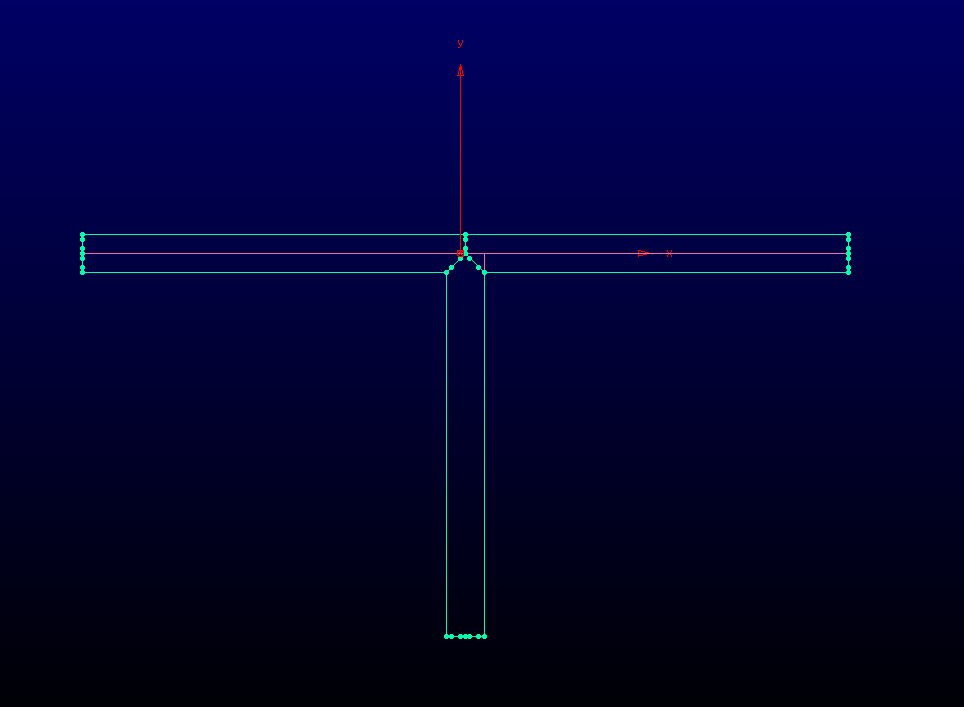
\includegraphics[width=50\unitlength]{./IMAGE/mesh/blocks_sketch}
            }
\put(70,0)  {
			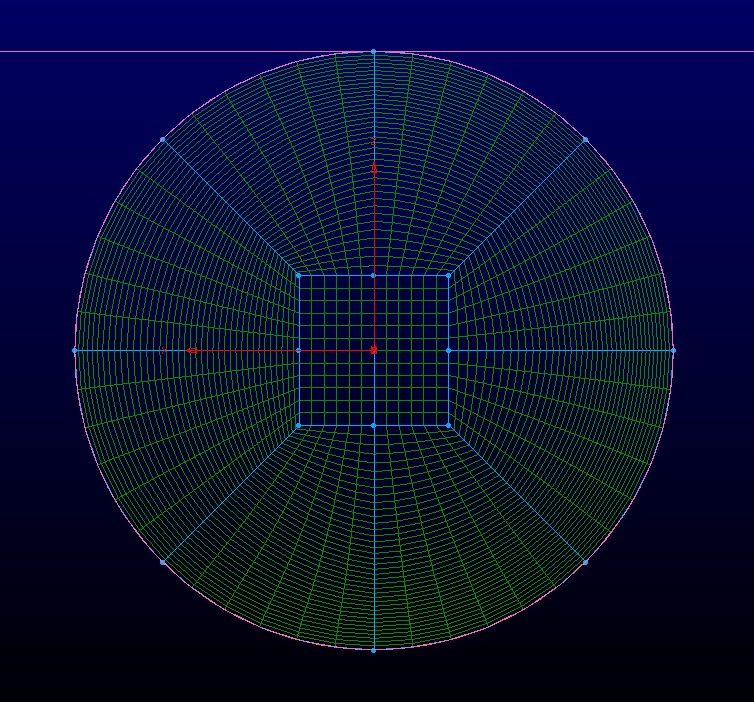
\includegraphics[width=40\unitlength]{./IMAGE/mesh/butterfly_noSolver}
			}
\put(5,20)  {a)}
\put(65,20)  {b)}
\end{picture}
}

\caption{mesh sketch: a) Division of the TJunction into three parts. Between parts we have an angle of $135^\circ$. b) A butterfly or O-H type mesh for cricular section meshing in which the central block mesh size will have influnce on mesh resolution in $\theta$ direction. A hyperbolic tangent distribution is applied in order to resolve boundary layer and a spacing constraint is set to the first cell size satisfying the criteria $y^+=1$} \label{mesh_sketch}
\end{figure}
}

\subsection{Pointwise(block or T-REX) snappyHexMesh (BoxRefinement)}

The mesh I'm using now is created by Pointwise using a hyperbolic tangent distribution function with one spacing constraint on the wall (imposing first mesh size) for which I don't know how much is the defaut streching factor. But hypertangent is often getting many points clustering close to the refinement region : we have 8 points in the viscous sublayer $y^+ < 10$.\\

I also tried snappyHexMesh using visualCFD (helpful for generating the snappyHexMeshDict) and managed to make a mesh with several boundary layers. Snappy is necessary if we want to have a refine region (Option existing : refinement regions - BoxRefinement). Refinement by region is not doable to my knowledge of Pointwise. \\

On the other hand, the meshes I created with T-Rex may actually work because we thought always there was something wrong with meshing. Well, there was until we get to relatively big Reynolds (there was a time that Re=1200 works while Re=2400 doesn't ... by memory, it's the one with a fillet but having very distorted cells). And when I continue to mesh with more cells, there comes the solvers constraint so not the problem with mesh. The current solver settings for $U\ p$ are much better than previous ones. I suppose old meshes with T-Rex may work and it's convenient if T-Rex works because even complicating the geometry (in the block meshing point of view) with a fillet, the mesh generation is practically the same/easy. And this may solve the problem with very big velocity at the corner. \\

Downside for snappyHexMesh \textcolor{blue}{Case Location on zaurak hluo/OpenFOAM/VE13} (they tell me snappy is really good at making cells orthogonal from the OpenFOAM forum of China) and T-Rex is that we lose the absolute control of every cell.  

\subsection{Mesh Setting in Channel Flow}
$\Delta x$ is a geometric serie $\iff$ $\Delta x$ is proportional to $x$

$\Delta x_1 = k x_1 + b$, $\Delta x_2 = k x_2 + b$ $\Rightarrow$ \\
$\Delta x_2 - \Delta x_1 = k \Delta x_2$ $\iff$ $(1-k)\Delta x_2=\Delta x_1$ \\

Alex, the one with linear relationship (necessity demonstration above, leave behind sufficiency...) that we saw the other day with the Channel flow (LES simulated by OpenFOAM) is indeed linear ($x$ vs $\Delta x$). In that case the total stretching factor (biggest comparing to smallest) is set to be 10.7028. Their mesh is created by blockMesh and strictly orthogonal. Mesh size in other two directions are repectively (for the finest simu): $\Delta x^+ = 9.88$ and $\Delta z^+ = 6.58$ and $\Delta y^+_0 = 0.47$ for the first cell.\\

\subsection{Standard procedure for cases}
How to do the cleansing of the mesh to clear out all possible errors systematically.\\

\begin{enumerate}
\item Estimate wall unity $\frac{\nu}{u_\tau}$ for first wall mesh size \begin{CJK*}{UTF8}{gkai} \textbf{计算进口流量,平均剖面,这样来确保至少 $u_\tau$ 和流量相容} \end{CJK*} 
\item Pointwise
	\begin{enumerate}
	\item Examine domains' aspect ratio see if it's symmetric 
	\item Select all connectors and apply equal spacing 
	\item Re-examine 1 
	\item Still not symmetric, cut the other half -> mirror -> merge -> apply spacing constraint to wall for first wall mesh size. 
	\item Check for mesh quality (Pointwise has different metrics to OpenFOAM's \textit{checkMesh}): aspect ratio, non-orthogonality, skewness... 
	\item CAE -> solver -> OpenFOAM 
	\item Delete ALL BCs and make new BC then select all blocks -> export -> CAE \\
	\end{enumerate} 

\item Before running simulation
	\begin{enumerate}
	\item \begin{CJK*}{UTF8}{gkai} \textbf{重要} \end{CJK*}  Rescale to meter : \textit{transformPoints -scale '(0.001 0.001 0.001)'} 
	\item \textit{checkMesh} 
	\item \textit{decomposePar} : run this interactively to see if it works as intended at the same time we can see output from my user-defined BC (useful). 
	
	\item \begin{CJK*}{UTF8}{gkai} \textbf{重要} \end{CJK*} Double check the solver used in \textit{sbatch} job submission file -> if needed add memory test (one-noed version or multi-noeds version). 
	\item In job submission file, check \textit{\$nos} \textit{\$logFile} numbering. Name the submission file using \textbf{8 chars}. 
	\item Final check for fluid properties and turbulence Model in \textit{constant}: $\nu$ or non-newtonian laws. \\
	\end{enumerate}

\item Simulation and postProcessing
	\begin{enumerate}
	\item Estimate simulation time -> choose queue -> Run simulation. 
	\item Monitoring log : Check CFL -> deltaT. 
	\item Monitoring log : Iterative sub solver performance : Iter* and residual for $(U\ p)$. 
	\item Visualization using paraview : python based (auto-determine machine zaurak/visu )
	\item Calculate $y^+ = \frac{u_\tau y}{\nu}$ a posteriori. 
	\item Using more cells number recalculate $y^+ = \frac{u_\tau y}{\nu}$ a posteriori \begin{CJK*}{UTF8}{gkai} \textbf{看看是否还需要再加密网格} \end{CJK*}. 
	\item Numerical scheme : time and space (less dissipative). 
	\item Check for max(U) at the corner. 
	\item Check for fluctuations at Dai's result using \textit{probes\_Dai} 
	\item Check for pressure solver abnormal behavior using \textit{probes\_pMonitor} 
	\item Check \textit{probes\_Port1\_and\_Port2} 
	\item \textit{sample -dict system/someDict} all \textit{timedir} for statistics 
	\item Field statistics like : turbulent kinetic energy, skewness (three components), dissipation rate. For convergence. Others : wall shear stress (viscous + turbulent) is constant in the whole boundary layer.
	\item Dissipation rate (a posteriori) determines K-scale $\eta_K$ which is critical for DNS -> reasonable MAX cell size. \\
	\end{enumerate}

\end{enumerate}

\begin{enumerate}
\item snappyHexMesh
\begin{CJK*}{UTF8}{gkai} 
\textbf{Hozlmann的tutorial(45DegreePipe)里面有先scale $1000$倍再rescale $1/1000$的过程,中间做snappy meshing,用一个bash script来完成的操作,具体原因未明} 
\end{CJK*}

\end{enumerate}

\section{Simulation cases}
\subsection{BC}
Try : \\
\begin{itemize}
\item[$\bullet$] \begin{CJK*}{UTF8}{gkai} 用压力差作为p边界条件比约束速度更容易收敛 \end{CJK*}

\item[$\bullet$] $\nabla p \cdot \vec{n}=0$ at all patches and add a reference pressure value somewhere in the tube to leave $p_{outlet}=10$ which may be too tight.=> \begin{CJK*}{UTF8}{gkai} 从微分方程的角度,在所有的边界上都需要有边界条件,加上pRef是为了求解二阶的泊松方程,从这个角度上述条件似乎讲得通。icoFoam tutorial cavity里除去没有进口条件(有速度在滑动壁面的条件->但这没有流量流进),跟上述p的BC设定是一样的,cavity里面fvSolution里面去掉pRef直接会报错。但我的case即使加上pRef,也会出现流量不守恒,但仅仅在求解p方程的时候出现。\textcolor{red}{怎么知道p的值,在预测步?具体流量怎么算的,这个应该不复杂} \end{CJK*} 

\item[$\diamond$] \begin{CJK*}{UTF8}{gkai} 进口条件里非流向的扰动是否被输运了?加和不加是不是一样,可以通过BC来测试,让流向生成两组同样的随机数,一组加非流向的扰动另一组不加非流向的扰动 \end{CJK*}

\item[$\diamond$] pipe flow with \textit{cyclic} BC \begin{CJK*}{UTF8}{gkai} 需要确定是否在网格生成的时候就需要设定好特定的除去cyclic的条件,neighbor是什么 \end{CJK*}

\item[$\diamond$] \textit{mapped} BC. Tutorial pisoFoam/les/ptizDaylyMapped. In blockMesh there is a offset which you can find in mappedPatchBase class.

\end{itemize}

\subsection{mesh}
Try : \\
\begin{itemize}
\item[$\diamond$] Use current solver settings to test T-Rex mesh ! Pipe or T.

\item[$\diamond$] \begin{CJK*}{UTF8}{gkai} SnappyHexMesh 逼近1.5M网格数 \end{CJK*} 

\item[$\diamond$] Poinwise solver to improve quality

\end{itemize}

\section{Boundary Layer Theory}

The way to determine wall shear stress $\tau_w$. There are two : \\

1. [Diagramme de Clauser] Knowing that mesuring the $U(y)$ distribution in the viscous sublayer ($y^+ < 3$) is extremely difficult, all mesurement is carried out in the log zone ($y^+ > 40$). We plot $\frac{U}{U_e}$ against $\frac{yU_e}{\nu}$. As soon as we get the plot, remembering the log-law :

$$\frac{U}{U_e} = \gamma (\frac{1}{\kappa} ln\frac{yU_e}{\nu}\gamma + C); \gamma = (\frac{C_f}{2})^{1/2}$$

which leads to actually a family of curves depending on $\gamma$. A simple fitting will deduce the value of $\gamma$ then $U_(\tau)$ then $\tau_w$ \\

2. Proposed by Kline et al. \cite{Kline1967}: Still mesuring the values in log zone, seeing that $U^+ y^+ = \frac{Uy}{\nu}$ retains true and  so when we get values of $U^+ y^+$ in the log zone we will have the left hand of $U^+ y^+ = \frac{y^+}{\kappa}lny^+ + Cy^+$ then solve for $y^+$ and then the corresponding $U^+$ which will leads to $U_\tau = \frac{U}{U^+}$ which should be a constant for all pairs of $(y^+, U^+)$ data we get. \\

\subsection{Questions on TBL}

According to Page 208 of Cousteix, in order for the log zone theory to hold, the zone must be somewhere between two scales i.e. $\frac{\nu}{U_{\tau}} \ll y \ll \delta$. Experience shows that log-law starts to be valid from $y^+ > 30$ and let's say $\frac{y}{\delta} < 0,1$ will make sense. Therefore $Re_{\tau} = \frac{\delta}{\nu/U_{\tau}} > \frac{10y}{1/30y} = 300$. In my case for $Re_R=2400, Re_{\tau} = \frac{0.0218*0.004}{10^{-6}}=87.2.$ \textcolor{red}{which is not good!} \\

And I didn't find the way to determine my boundary layer thickness. \cite{Purtell1981} maybe helpful giving out the percentage of log-zone in a boundary layer.\\

Roussel \cite{Roussel2016} has iterative procedure to determine the right profile. \textcolor{red}{this is for profile in the boundary layer}. His precedure : \\
1. Knowing the $\delta_{in}$ at the inlet estimate $X_0$ which is the position from the leading edge. \\
2. $\delta_{in} \Longrightarrow \delta(x) \Longrightarrow Re_{\delta(x)}$
3. Using $\delta(x) and Re_{\delta(x)}$ at specific position $x$, estimate $u_\tau$ by firstly guessing or by abaque have a $c_f^{(0)}$ then we will have a guess of $u_\tau$. \\
4. Using classic results inside the boundary layer mean profile along with the external flow with $u_\infty$, calculate the thickness $\theta$ then estimate $c_f^{(1)}$ with eq. (3.13). \\
5. Getting $c_f^{(1)}$ means getting a new $u_\tau$ because $c_f = \frac{\tau_w}{\frac{1}{2}\rho u_\infty^2}$ and $\tau_w \Longrightarrow u_\tau$\\
\textcolor{red}{How can I do this without knowing $\delta_{in}$ ???}\\
HuangGang \cite{huang2015} mentioned a weighting function
$$W(\eta) = \frac{1}{2} [1+ tanh[\frac{a(\eta-b)}{(1-2b)\eta+b}]/tanh(a)], a = 4, b = 0.2$$ which uses $\eta$ as variable and $\eta$ can be bigger than $1$ : outside the boundary layer. \textcolor{green}{Wu Jianzhao tells me that he acutally have a $\delta_{in}$ at the entrance. And I don't see how should I figure it out refering to Dai.}

\section{skip this part for now}

simScale has a turbulent pipe flow tutorial \\

Timofey Mukha did channel flow systematically with OpenFOAM. Many LES models.\\

Testing DNS capability of OpenFOAM and STAR-CCM+ didn't give any indiction of inlet condition by my memory \\

This guy \cite{EugeneThesis2006} used mapped inlet and This theis used OpenFOAM. He is on the cfd-forum. pdf on my disk biblio/thesis.\\

Study on rectangular Tjunction. \cite{Fukushima2002} experiement. Numerical \cite{Georgiou2017}

\section{biblio}
\subsection{Pipe Flows}
\subsubsection{Experiment Toonder1997 \cite{Toonder1997}}
Using two dimensional LDV mesurements, turbulence statistics like mean profile and rms is Reynolds dependent scaled on inner variable $u_\tau$ in range Re $5000 -25000$. $u_\tau$ is estimated by mesuring pressure drop. \\

For the mean profile :\\
The constant $B$ in $U^+_z = Alny^++B, if y^+>30$, for high Reynolds number like at least $Re>10000$, $B=5.0$. However for low Reynolds number $Re=4900$, $B=5.5$ which is recommended in my Reynolds $2400, 4000, 10400$ by Kim et al. \cite{KJM1987}. \\

For RMS and Reynolds stress : \\
$rms(U^+_z)$ shows Reynolds dependancy in $y^+ > 30$ while $rms(U^+_r)$ has a much more visible Reynolds dependancy. Fig15 shows that turbulent stress drops until we hit the cylinder center which is $y+=170 for Reynolds=4900$ as in caption of Fig5 indicated. \textcolor{red}{So I'm assuming that the the whole pipe is in the boundary layer ??? There is no external flow ??? If yes, my Re2400 case should be too. And it is as I use the mean profile and RMS fluctuation enveloppes. But contradicts with the critera mentioned in Cousteix'book $Re_{\tau} > 300$}

\section{big picture}
Dai has experiment and Fluent data. I must compute a better result using OpenFOAM.\\




\newpage
\bibliography{workFlow}
\bibliographystyle{ieeetr}

\end{document}
